\chapter*{About this project Abstract}

\bigbreak
The project aim is to create booking system for Bank of Ireland workbenches as its becoming more and more automated all branches across Ireland have viewer people in them and all the free space become available and unused so workbenches idea was introduced to fill the empty space. The approach taken to develop this was make a web application using MEAN (MongoDB, Express, Angular, Node) approach
and swap MongoDB for Firebase. Conclusion was reached after much research to develop 2 websites one for the users one for the admin. The purpose of admin website is to add new workbenches all across Ireland and be able to edit them and suspend them if needed. The user site has authentication from third party software called Auth0 system them lets them log with gmail or GitHub for convenience or sign up for an account in and see all the workbenches added and lets them book and workbench available as well as search for viany particular workbench in the Country, google Maps plug in is also available that shows all the workbenches on map marked with pin that displays additional details. The finished websites were uploaded on heroku server so can be accessed publicly.
Firstly, at the moment, users must contact the workbench only during business hours to schedule a room. As the project proposes an online booking system, it will be available 24/7, thus solving this issue and cutting out the middle-man as the workbench does not need to be contacted directly.
The project also enables the user to see all centres on a map within a specified distance. It will act as a 'one-stop shop' for the user, rather than having to contact each centre separately to check availability or to make a booking. As well as this it will display to the user alternate centres if one is not available. The application allows workbenches to be easily added, edited or removed as needed.


\chapter*{Authors}
Developers of the project were:
\bigbreak

Vytas Vaiciulis 
\\Niall Mcgrath 
\pagebreak

\chapter*{Acknowledgements}
We would like to acknowledge team supervisor Damien Costello for support and understanding as well as all GMIT teachers for helping us to get this far.
\pagebreak


\chapter{Introduction}
\bigbreak

The approach taken to develop this was make a web application using MEAN (MongoDB, Express, Angular, Node) approach and swap MongoDB for Firebase. Conclusion was reached after much research to develop 2 websites one for the users one for the admin. The purpose of admin website is to add new workbenches all across Ireland and be able to edit them and suspend them if needed. The user site has authentication from third party software called Auth0 system them lets them log with gmail or GitHub for convenience or sign up for an account in and see all the workbenches added and lets them book and workbench available as well as search for any particular workbench in the Country, google Maps plug in is also available that shows all the workbenches on map marked with pin that displays additional details. The finished websites were uploaded on heroku server so can be accessed publicly.
Model View Controller was used in the development of this website as it separates all 3 components. So Firebase was chosen for Mode to store all the workbench data JavaScript controllers to manipulated  filter and do the logic and html to display element for the user as booth  websites bookAroom-user and bookAroom-Admin connect to same database but are restricted to certain capabilities. One of the requirements were that application need to be accessed by all different platforms research literature review was carried out in cross platform development and conclusion was reached to develop it as web application as it cross platform accessible as well as cross screen accessible with aid of bootstrap.
This project was developed to create an easy way for a user to book a room in an Innovation Centre, or more specifically the Bank of Ireland Workbenches. There are a number of reasons why a system like this is needed.
Firstly, at the moment, users must contact the workbench only during business hours to schedule a room. As the project proposes an online booking system, it will be available 24/7, thus solving this issue and cutting out the middle-man as the workbench does not need to be contacted directly.
The project also enables the user to see all centres on a map within a specified distance. It will act as a 'one-stop shop' for the user, rather than having to contact each centre separately to check availability or to make a booking. As well as this it will display to the user alternate centres if one is not available. The application allows workbenches to be easily added, edited or removed as needed.



\chapter{Context}
\begin{itemize}
\item Provide a context for your project.
\item Set out the objectives of the project
\item Briefly list each chapter / section and provide a 1-2 line description of what each section contains.
\item List the resource URL (GitHub address) for the project and provide a brief list of the main elements at the URL.
\end{itemize}

\section{Filler}


\section{Filler}


\chapter{Methodology}


\section{Agile}

During this project, the agile approach was chosen over more traditional approaches like the waterfall model or other sequential approaches for its flexibility. This approach helps respond effectively to change through incremental, iterative phases (called sprints), which seemed more effective than the waterfall methodology which relies on every requirement being known before any design or coding occurs. A Scrum methodology was used so that each phase included all aspects of development. Using this approach, small changes were added each phase to improve it.

\section{GitHub}

At various times throughout the project, GitHub, an online project hosting tool, was used to maintain and keep track of the development. GitHub was chosen as it offers all the distributed revision control and source code management functionality of Git but has other benefits which make it easier to use such as a web based interface and desktop integration, rather than just using the command line. Here are the repositories links that the project is composed of. 

https://github.com/VytasHub/bookAroom-user
https://github.com/VytasHub/bookAroom-admin
https://github.com/mcgrath94/FYP-Google-Maps
And also link to the documentation repository.
https://github.com/VytasHub/final-year-project-template



\section{CROSS-PLATFORM DEV}

There are a number of reasons a web application was selected over a native app. Web applications have the benefit of portability as they can be coded once and ran on many different devices rather than having to waste time and effort developing on multiple platforms. In a similar way, this makes the maintainability of a web app easier. Naturally these two factors mean they are more cost effective. Web apps also do not require the user to download or update them. Although web apps have some drawbacks such as not being able to achieve the same performance or user experience as native apps, there is little performance penalty for apps that aren't graphic heavy. 

\section{Testing}

The app was tested by running it locally and listening to that port. This allowed to fix any errors and verify the application was in working order. It was also tested from various locations to determine how accurate it was at finding the users location.




\chapter{Technology Review}
\section{Development Environment}
About seven to ten pages.
\subsection{Debian}
\bigbreak
Debian is an open source operating System developed. It’s one of many distributions of Linux but is one of the earliest distributions and was first announced in 1993 by Ian Murdock. It requires small hardware resources to run and is easy to set up and install it has graphical user interface version as well as command line version which father. When distribution is released initially it’s marked as unstable, father sufficient amount testing is done it become as stable and usually is adopted by more people than because it has less bugs and is more reliable. Debian has access to over 50 000 to packages located on the internet and any package can be installed with one command line which makes ideal work environment for web development because web development relies on many different components put together and if not done right issues arise with dependencies etc. With commands like sudo apt-get you can install any package you want and well documented and big community behind it.Tools like npm Node packet manger and grunt work very well in this environment.

\subsection{Cli and Gnu Nano}
\bigbreak
Command Line Interface (CLI) doesn’t come with Debian it has to be installed. Moust of Operating Systems come with many tools installed which makes them very big and a bit slow Operating System like Debian takes different approach and start with just essential tools and then you install only tools that you need. CLI is needed to install some packages and execute some of the commands in Debian when working web environment.GNU Nano is a text editor Unix like operating system which makes it ideal for Debian and all Linux distributions. It allows for convenient bash scripts to be set up while in command prompt or terminal as now in Debian. As well it allows for convenient GitHub commits you can enter commit message and press chines hat and O to write out and commit changes to github.


\subsection{Npm/Bower Grunt}
\bigbreak
These two tools are absolutely essential to web development environment and you are must like wouldn’t be able to develop without them in today’s world. Npm is a default manager for JavaScript runtime environment in Node.js.it manages all package dependencies of an application as well as installing them. Grunt makes web development environment more efficient by eliminating repetitive tasks such as unit testing as well as shortening your run scripts such grunt serve is very popular for running your application as that is very repetitive command and is executed a lot.


\bigbreak

Bower its package management system for web applications and uses node.js and npm.
In this project bower installation method was used preferably to npm. When installing firebase to the application throw npm using commands like.

\begin{itemize}
	\item npm install firebase –save
\end{itemize}
Reference needs to be added to index.html page which downloads firebase module over the net.


\begin{minted}{javascript}
src="https://cdn.firebase.com/js/client/2.2.4/firebase.js"
\end{minted}




\subsection{Github, git}
\bigbreak
Github was founded in 2008 its web based git repository it lets users have public repositories which are free and you can have any amount it also has an option for private repositories for which you have to pay and the more private repositories you have more you have to pay, but I has student bundles which provide 100 dollars’ worth of development tools which is great for beginner developers such as myself. It provides graphical user interface for Windows and Mac to manage maintain and update projects but it does cause some errors failing to commit or failing to push or merge when that happens user is suggested to use git to fix the errors. For that reason git is way more stable and reliable which is command based tool it has five major commands hat are used constantly.It has played major role in this project and made project way more manageable and sustainable as well as less error prone regular commits made sure of small incremental progress throw out life of the project.

\begin{itemize}
	
\item git clone path/to/repo \\
\\This command allows to clone any project from your github account or any publicly available project for that matter.

\item git status \\
\\Checks the status of project once it has been cloned it shows added deleted and modifies files as well as indicates which files are tracked.

\item git add . \\ 
\\Add folders or files to be tracked by github so later they can be committed and pushed on to github account.

\item git commit –a \\
\\Makes local commit of all the changes done in folder added by previous command git add .

\item git push origin master \\ 
\\ Pushes commit (git commit -a) to users github account on his/her account

\end{itemize}


\subsection{Sublime, Live Reload and Chrome}
\bigbreak
Sublime is code editor that supports cross platform functionality. It supports many different programming languages as well as mark-up languages and functionality can be extended with huge amount of plug in packages available. Currently Sublime is on version 3 it has been released in 2013.
There are other editors out there such as Notepad++, Brackets, Vim Atom but Sublime proved to be most efficient in web development environment.Some of its best features;

\begin{itemize}
	
	\item auto safe 
	\item autocompleting 
	\item multi-select-editing 
	\item spell check 
	\item snippets  

\end{itemize}





\section{Mean Stack}
\subsection{Mongodb/Firebase}
\bigbreak
MongoDB comes as part of popular stack MEAN it’s a cross-platform document-oriented database and is classified as NoSql database. Its free and open source under a combination of the GNU Affero General Public License and the Apache License. Being object oriented data base it is shameless and needs no scheme as its older counter parts SQL based data bases. For that matter there is mongoose was developed which is an ORM for Mongo and is written in node.js and allows to give mongodb a scheme to make it more comparable with older system which all use SQL based data bases. It has grown in popularity and now is fourth most popular database management system. Its stores everything as an object in JSON like format and files object are indexed which allows instant retrieval of an object. 
\\
\bigbreak
Firebase was founded in 2011 and is object oriented database allowing for fast retrieval of objects. It allows to store and sync data across many different platforms one of its best feature is three way data binding between Firebase and your applications view and controller and stores data in json like format which is well understood format by developers across the world. Company has been acquired by google in 2014. Firebase is built in to Auth0 authentication framework which was one of the reasons why it was chosen for this project because Auth0 framework was used for authentication of this application Auth0 framework will be explained in more detail in Components section. Firebase generates authentication key which needs to be supplied to Auth0 in order to let firebase requests throw authentication system shown below.
\begin{minted}{javascript}

var ref = new Firebase("https://bookaroomfirebase.firebaseio.com/");
ref.auth("AUTH_TOKEN", function(error, result){
if (error){
console.log("Authentication Failed!", error);
}else{
console.log("Authenticated successfully with payload:", result.auth);
console.log("Auth expires at:", new Date(result.expires * 1000));
}
});

\end{minted}


\subsection{Express}
\bigbreak
Is part of the MEAN stack bundle and it handles server side. Express is owned by IBM as of 2015 ans in 2016 IBM announced that it will put Exprrss.js under the stewardship of the Node.js foundation incubator.
\bigbreak
Express.js is a node.js web application (node.js is covered in other section) and uses minimalistic approach all server side script can be done in few lines of code this peace of code was used to run bookAroom-admin website shown below.

\begin{minted}{javascript}

var express = require('express');
var app = express();
var port = process.env.PORT || 8080;

app.use(express.static(__dirname + '/dist/'));

app.listen(port, function() {
console.log('Our app is running on port: ' + port);
});

\end{minted}
\bigbreak
And everything else is available as a plug in you simply require all the modules that you need. The modules below where used in bookAroom-user application to authenticate user.

\begin{minted}{javascript}

var http = require('http')
var cors = require('cors');
var jwt = require('express-jwt');
var dotenv = require('dotenv');

\end{minted}


\subsection{Angular}
\bigbreak
Web applications are browser-based applications running in a browser
using HTML5. WebHooks allow developers to access the hardware on a
phone, this was unavailable before HTML5 [16], also it allows other features
such as web storage, indexed database APIs, file APIs, web SQL Databases and
Offline Web GeoLocations [16]. This makes web applications more mobile
friendly and compatible and allows them to use the full range of phone
features. They do not require installation or any upgrades as it contains a one
to many relationship (one server, many clients) so any updates are done on
the server side and all clients get updated, but the network is required at all
times in order to access the application. It lacks the native look and feel of
target platforms such as Android, iOS or Windows Phone, altough there are
many tools out there trying to solve the problem by simulating a native look
such as Xui, JQyeryMobile, Sencha Touch, JQTouch and WebApp.net. Some
6
frameworks developing web applications include AngularJS, Ruby on Rails,
Django and Drupal. AngularJS is explained in more detail down below.
\bigbreak
It was developed by Misko Hevery in 2009 at Brath Tech LLC. It is now an
open source framework mainly used for developing single page applications
(SPA) it has become widely well known and is the top choice for many
developers for creating dynamic html pages. In order to be able to program
in AngularJS you have to know HTML, CSS and JavaScript. It is maintained by
Google and the developer-community; it is under MIT license [17]. It uses
data binding which means you can attach controllers to certain parts of the
page as well as taking advantage of the MVC (Model, View, Controller)
pattern, creating a loosely coupled design to separate the three components
of the web application so that they all are independent to one another; one of
them can be changed without impacting the others and you can swap and
change components. If an application contains more than one page it can use
Client side routing in order to dynamically switch content without refreshing
the page [18]. The Batarang plugin was built by Google in 2012 to improve
the debugging of web applications built using AngularJS. It is also used with
another three popular technologies known collectively as the MEAN Stack
(MongoDB, Express, AngularJS and NodeJS). MongoDB is cross platform
oriented database, it uses a JavaScript/JSON style syntax; it is open source.
Express is a server framework that is used for building single page web
applications and is expandable via plugins. NodeJS is cross platform runtime
environment for server side applications, it’s open source. As we can see all
the technologies used in the MEAN stack are open source suggesting the
reason for its huge community and popularity.

\subsection{Node}
\bigbreak
Is an open source cross platform runtime environment for developing server-side web applications. It has been founded and released in 2009 and interprets googles V8 JavaScript engine. Some of the corporate users from industry include IBM, LinkedIn, PayPal, SAP, Yahoo so it’s well adopted by heavy hitters in industry. Originally Node.js was only supported by linux operating systems, which enforces the reason for using Debian/linux operating system for this project.


\section{Components}
\subsection{Yeoman/Modules}
\bigbreak
Yeoman is an open source client side development stack allowing developers web applications quickly not worrying about initial process of setting up it includes all industry standards such bootstrap responsive design etc. Some of the tools used in conjunction with yeoman generator.

\begin{itemize}

	\item Grunt 
	\item Gulp
	\item Bower
	\item Npm

\end{itemize}

When yeoman generator is initialized it generates full web application with all of the main structure. 
It generates app.js file which contains all the modules injections and any new injections need to be added to this file some of the modules used in this project:

\begin{itemize}
	
	\item 'firebase' 
	\item 'ngCookies'
	\item 'ngResource'
	\item 'ngRoute'
	\item 'ngSanitize' 
	\item 'ngTouch'
	\item 'formly'
	\item 'formlyBootstrap'
	\item 'ngAnimate'
	
\end{itemize}
\bigbreak

As well it contains Route Provider that maps all the views html pages to JavaScript controllers so each view is served one controller JavaScript class, this might prove a problem as it only allows for one script per class so services can be injected to controllers to add more scripts per one view.It also maps pages html address so this can be used in future for authentication.Code below how routing ow one html page looks like.
\bigbreak
\begin{minted}{javascript}

 .when('/view', {
 templateUrl: 'views/view.html',
 controller: 'WorkBenchController',
 controllerAs: 'fireApp'
 })

\end{minted}
\bigbreak
Testing modules of Yoeman:
\bigbreak

\begin{itemize}
	
	\item jshint 
	\item travis
	\item karma
	\item jscsrc
	
\end{itemize}
\bigbreak

JSHint, a tool that helps to detect errors and potential problems in  JavaScript code.
Karma a simple tool that allows you to execute JavaScript code in multiple real browsers.
Travis lets you test your build modules.






\subsection{Angular formly}
\bigbreak
Angular formly simplifies form layout in html and allows for more structured code give forms consistency, flexibility, maintainability, simplicity and sanity. Before Angular-formly if you would wanted to have a form you would had something like this to get your input from user:

\bigbreak
\begin{minted}{html}

<form>
<div class="form-group">
<label for="exampleInputEmail1">Email address</label>
<input type="email" class="form-control" 
id="exampleInputEmail1" placeholder="Enter 
email" ng-model="vm.user.email">
</div>

<div class="form-group">
<label for="exampleInputPassword1">Password</label>
<input type="password" class="form-control" 
id="exampleInputPassword1" placeholder="Password"
 ng-model="vm.user.password">
</div>

<button type="submit" class="btn btn-default"
 ng-click="vm.submit(vm.user)">
 Submit</button>
</form>

\end{minted}
\bigbreak
For every bouton check box dropdown list etc you need a div with at-least 3 lines of code formly replaces that with this:
\bigbreak

\begin{minted}{html}

<formly-form model="vm.user" fields="vm.userFields">
<button type="submit" class="btn btn-default" 
ng-click="vm.submit(vm.user)">Submit</button>
</formly-form>


\end{minted}
\bigbreak

Which is efficient from html point of view but it does call additional JavaScript so it trims down on html but beefs up on server side. Depending on the application this can be used or not. But it does make html more readable and understandable.




\subsection{Ng-repeat, orderBy, filter}
\bigbreak

All of the more advanced applications today have some sort of dynamic element to it there is very few simple static content websites. Websites today are dynamic and ever changing the dynamic element of the websites always includes some sort of connections to database might be sql, object oriented or graph database it calls thouse elements from database and must render them in html and css rendering each element manually would be tedious and time consuming ng-repeat allows to define html once for one element and looped throw all the elements using same code and it looks like this:
\bigbreak

\begin{minted}{html}

<tr ng-repeat="item in WorkBenches | orderBy:sortType:sortReverse | filter:searchWorkbench">
<td>{{ item.Address }}</td>
<td>{{ item.CityTown }}</td>
<td>{{ item.WName }}</td>
<td>
</tr>

\end{minted}
\bigbreak

So with some JavaScript code it makes call	to Firebase database and for every item in WorkBenches which we can see there a few t renders it in html.
\bigbreak

\begin{center}    
	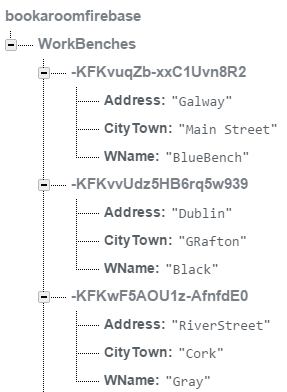
\includegraphics{img/FirebaseLayout.png}
\end{center}
\bigbreak

And the effect of ng-Repeat in html page is this and you can have as many elemnts as you like.

\begin{center}    
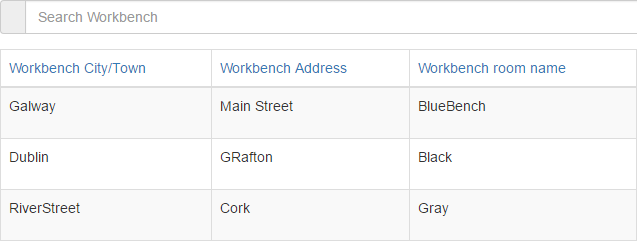
\includegraphics{img/PrintOutHtml.png}
\end{center}
\bigbreak

Few of other elemnts to mention is orderBy and filter. Orderby alows to order item in ng-repeat so you can order by any of the three atributes; Address, CityTown, WName. Filter alows to to add search bar to the list so you can look for item so as you type in name you looking for only thouse item containg typed in cahracters get renderd in html and if search bar is empty all items are rendered because all contain nothing. Ng- Repeat just makes life easier.




\subsection{Heroku}
\bigbreak

  Orion Henry, Adam Wiggins and James Lindenbaum founded Heroku in 2007 and was acquired by Salesforce in 2010.Heroku is cloud based Platform-as-a-service for short is called PaaS in the beginning it supported just Ruby but now since it grew so in popularity it supports more languages like; PHP, Go, Java, Scala, Clojure, Python and most important Node.js which made it possible to develop this application.Few things are needed to get started with heroku
\bigbreak
\begin{itemize}

	\item Node 
	\item Npm
	\item Heroku Toolbelt
	\item Git Bash
	
\end{itemize}
\bigbreak

After these tools are installed in command prompt you type in heroku and then heroku login that will give you powers to upload your website from command line from your git repository.

You will need to create proc file in your root repository and include this peace of code to tell heroku server to run your application just same way you start your application locally same way it start on Heroku server you just need to tell it.

\bigbreak


\begin{itemize}
	
	\item web: node server.js

\end{itemize}
\bigbreak

When you are loged in your heroku account throw cmd you need cloned git repository using git command (This emplies your application has node server build)
\bigbreak

\begin{minted}{html}

$git clone https://github.com/VytasHub/bookAroom-admin

\end{minted}
\bigbreak

You than go heroku create that creates your website.Afther that you type following command which gives website name nad port number on which it listens. 

\bigbreak
\begin{minted}{html}

heroku apps:rename heroku-node-8080 --app calm-reaches-6216

\end{minted}
\bigbreak

Than you simply push to server and your app is runing.
\bigbreak
\begin{minted}{html}

git push heroku master

\end{minted}
\bigbreak

Few other usefull commands to mention.This will alow to see you if the application is running.

\bigbreak
\begin{minted}{html}

$ heroku ps:scale web=1

\end{minted}
\bigbreak

And this will open website from command line.

\bigbreak
\begin{minted}{html}

$ heroku open

\end{minted}
\bigbreak

One of the issues that occurred while deploying to server was when pushing to server using git push heroku master old website were getting pushed. So need to use git status to see what you actually pushing because git repositories get queued in heroku and only first one gets pushed.

\subsection{Auth0}

\begin{minted}{javascript}

.when('/view', {
templateUrl: 'views/view.html',
controller: 'WorkBenchController',
controllerAs: 'fireApp'
})

\end{minted}








\chapter{System Design}
\section{bookAroom-user}
\bigbreak

We have five components to the application

\begin{itemize}
	\item Auth0
	\item Firebase
	\item MongoDB
	\item WebApplication 
	\item Social Providers
	\item Heroku
\end{itemize}
\bigbreak

Down below flow diagram of the application is displayed.

\begin{center}    
	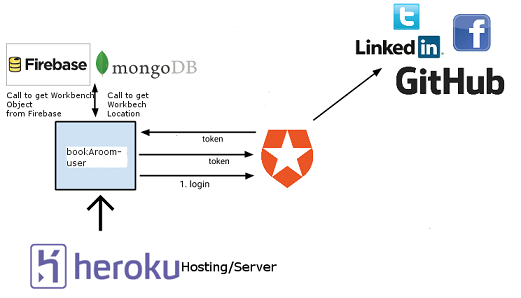
\includegraphics{img/userFlow.png}
\end{center}
\bigbreak


\subsection{Auth0}
Auth0 logging in system which allows user to sign up or log in with social provider such GitHub or Gmail. And is composed of 2 part an Angular app which contains all of the websites content and a node API which handles the logging , but when uploading it to heroku server prove to be challenging to start 2 separate components so bout were combined into one server.js file.
\bigbreak

\begin{minted}{javascript}

var http = require('http');
var express = require('express');
var cors = require('cors');
var app = express();
var jwt = require('express-jwt');
var dotenv = require('dotenv');

dotenv.load();
var port = process.env.PORT || 3001;

\end{minted}

\bigbreak

Auth0 system had to be configured by adjusting following variables in auth0-variables.js calss. The variables show below were obtained from Auth0 provider when crating the application.

\begin{minted}{javascript}

var AUTH0_CLIENT_ID='d4aV2GYuoQxjQ4qU5yfS3XiIQPwdmkOH';
var AUTH0_DOMAIN='book.eu.auth0.com';
var AUTH0_CALLBACK_URL=location.href;
var AUTH0_CLIENT_SECRET='78KGRbG59R-
FEevfFL8eIBeGt2bf3DucmAMqeLzuv4jpbGnM-uoXiea_EqZoWyLN';


\end{minted}
\begin{center}    
	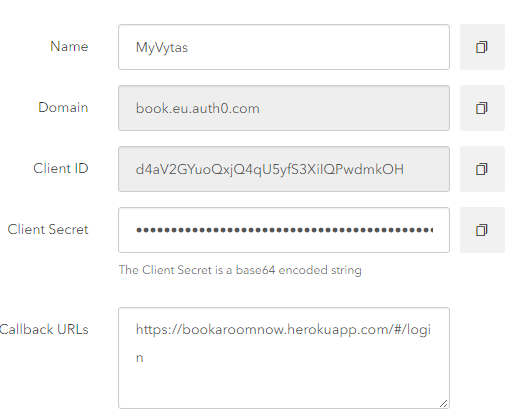
\includegraphics{img/AuthProfile.png}
\end{center}


\pagebreak
\subsection{Firebase}
\bigbreak
Firebase store all the workbeches object and can be Created, Updated, Deleted.

\begin{center}    
	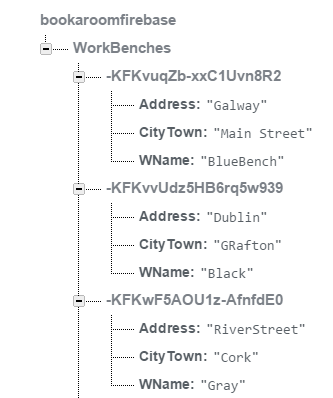
\includegraphics{img/Firebase.png}
\end{center}
\pagebreak





\section{bookAroom-admin}
As many pages as needed.


\chapter{System Evaluation}
As many pages as needed.
\begin{itemize}
\item Prove that your software is robust. How? Testing etc. 
\item Use performance benchmarks (space and time) if algorithmic.
\item Measure the outcomes / outputs of your system / software against the objectives from the Introduction.
\item Highlight any limitations or opportuni-ties in your approach or technologies used.
\end{itemize}

\chapter{Conclusion}
About three pages.

\begin{itemize}
\item Briefly summarise your context and ob-jectives (a few lines).
\item Highlight your findings from the evalua-tion section / chapter and any opportuni-ties identified.
\end{itemize}

